\section{Reverse\_Shell}

\begin{center}
    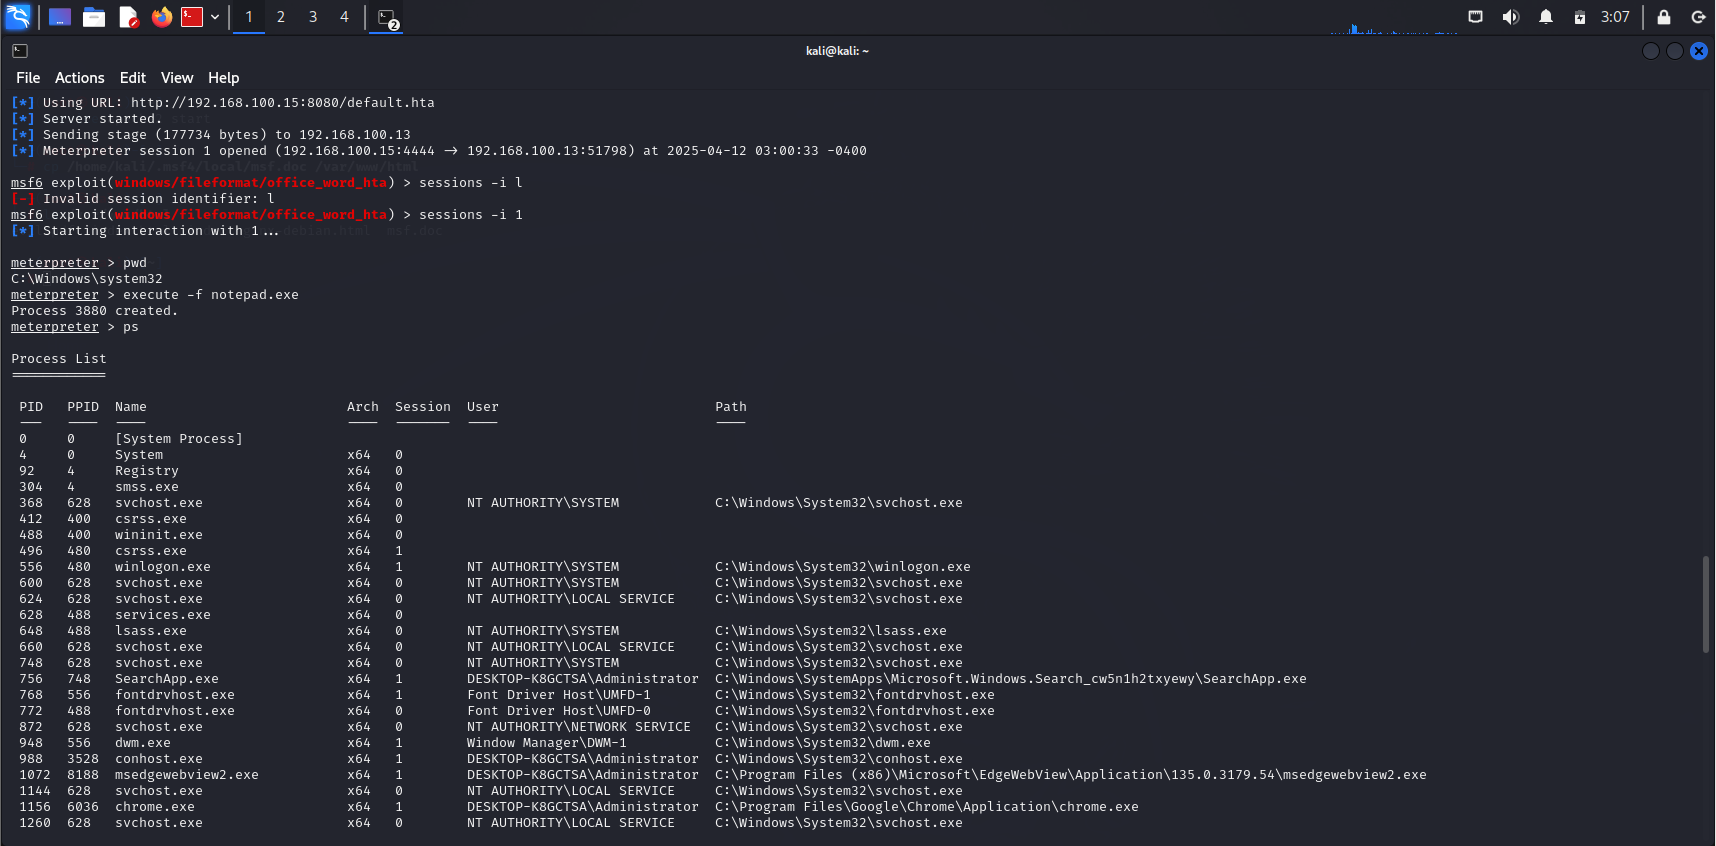
\includegraphics[width=0.8\textwidth]{Question/SC/ps.PNG}
\end{center}

\vspace{0.15cm}

\begin{center}
    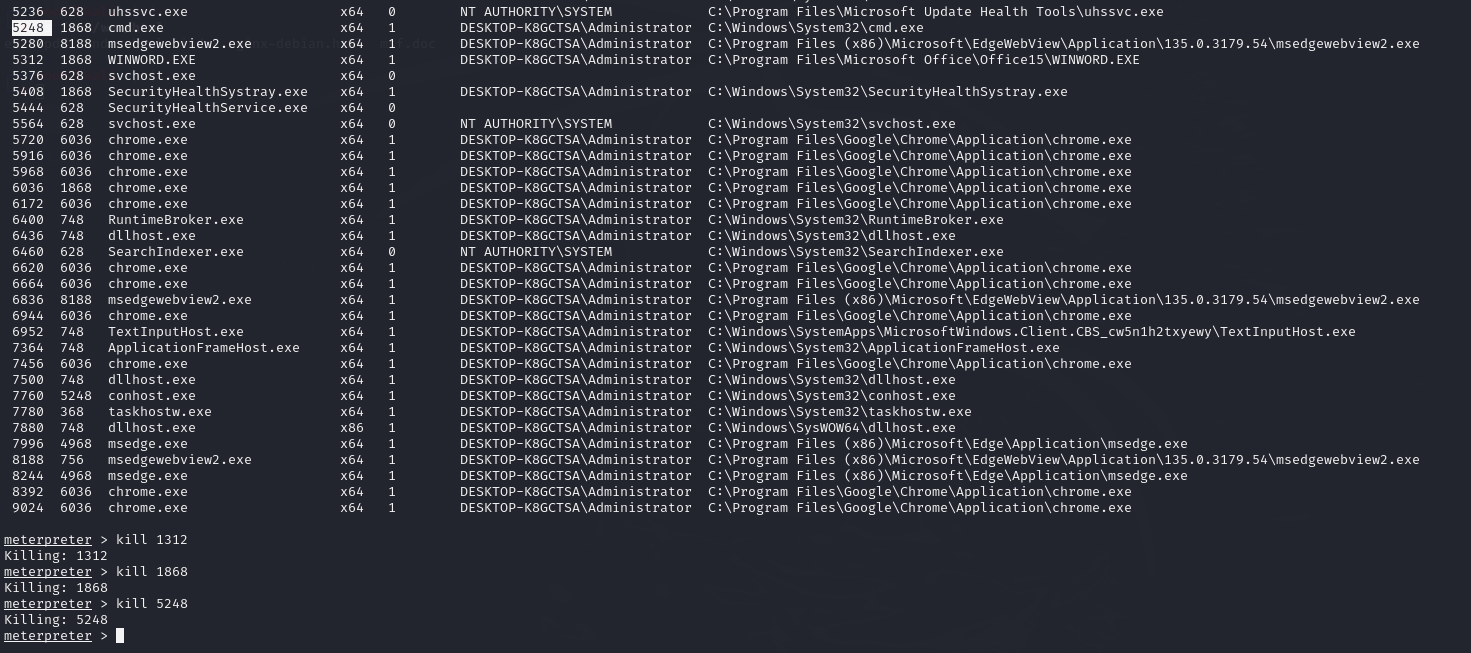
\includegraphics[width=0.6\textwidth]{Question/SC/kill_kali.PNG}
\end{center}

\vspace{0.15cm}

\begin{center}
    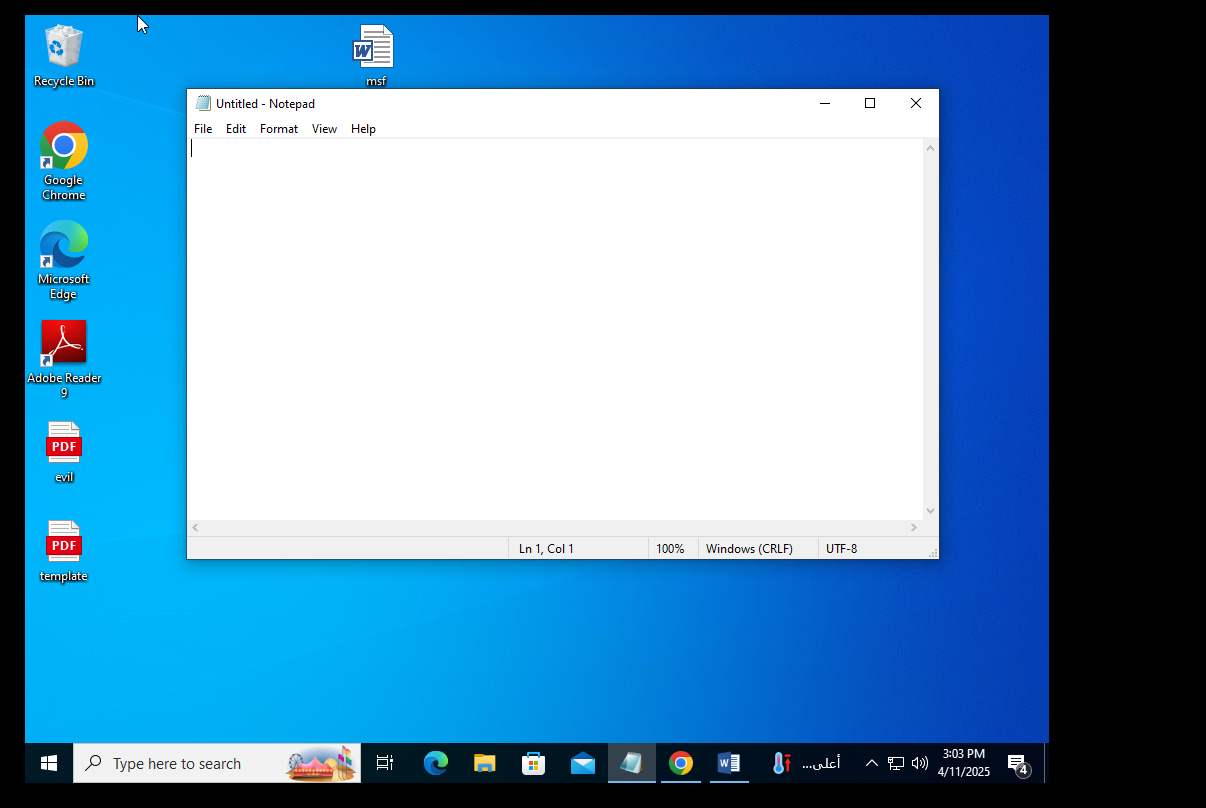
\includegraphics[width=0.6\textwidth]{Question/SC/kill.PNG}
\end{center}


\vspace{0.35cm}


\begin{prettyBox}{Remarque}{myblue}
    \begin{itemize}
        \item Après que l'utilisateur ouvre le fichier \texttt{msf.doc}, le payload s'exécute et l'on peut alors démarrer une session de type \texttt{reverse\_shell}.
    \end{itemize}
\end{prettyBox}

